% ----------------------------------------------------------------
% Article Class (This is a LaTeX2e document)  ********************
% ----------------------------------------------------------------
% xelatex
%\documentclass[12pt]{article}
\documentclass[UTF8,12pt]{ctexart}
%\usepackage[UTF8]{ctex}
%\usepackage[english]{babel}
%\usepackage{amsmath,amsthm}
%\usepackage{amsfonts}

\usepackage{graphicx}
\usepackage{hyperref}
\usepackage{caption} %figure环境下自动加的图标号怎么去掉?caption*{}

\usepackage{amsmath}
\usepackage{subfigure}
\usepackage{amsfonts}
\usepackage{amsthm}
\usepackage{mathrsfs}

\graphicspath{{Figures/}}

%% THEOREMS -------------------------------------------------------
%\newtheorem{thm}{Theorem}[section]
%\newtheorem{cor}[thm]{Corollary}
%\newtheorem{lem}[thm]{Lemma}
%\newtheorem{prop}[thm]{Proposition}
%\theoremstyle{definition}
%\newtheorem{defn}[thm]{Definition}
%\theoremstyle{remark}
%\newtheorem{rem}[thm]{Remark}
%\numberwithin{equation}{section}
% ----------------------------------------------------------------
\begin{document}

\title{技术报告\\-Paper Machine Pipeline}%
\author{刘维湘---深圳大学}%

%\address{中国北京}%
%\thanks{感谢2019冠状病毒,让我们认清了世界的本质.本外传所有资料来在网络,若有侵权,请提出。书中观点仅代表个人成见,欢迎讨论交流。本资料仅只能用于非商业用途;若发现侵权,我们有捍卫自身权益的权利。}%
\date{20201212}%

\maketitle
% ----------------------------------------------------------------
\begin{abstract}
科学与技术的发展离不开实践与思考。个人的学习笔记有利于自己系统的思考,为了更好地实践、交流与传承。\footnote{源于个人日常学习中的点滴积累。很多资料来自网络。仅可用于非商业目的教学与研发。}

\end{abstract}

\newpage
\begin{figure}[h!]
\begin{center}
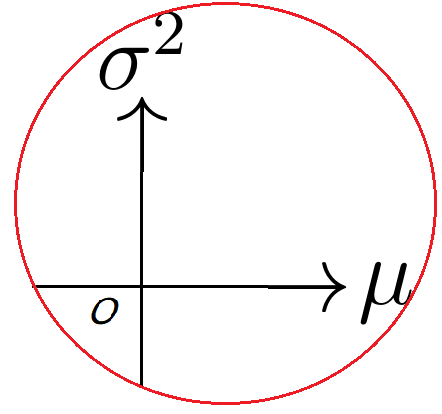
\includegraphics[width=12cm,height=12cm]{mu_sigma.png}% This is a *.eps file
\end{center}
\caption*{概率分布的空间(以正态分布为例)}\label{NLP}
\end{figure}


\newpage
\tableofcontents

\newpage
% ----------------------------------------------------------------
\section{描述问题}

\subsection{应用背景}

\subsubsection{是基础科学问题}

\subsubsection{或是工程应用问题}

\subsubsection{或是应用基础研究问题}

\subsection{研究现状}

\subsubsection{国外现状}

\subsubsection{国内现状}

\subsection{存在不足}

\newpage
\section{建立模型}

\subsection{出发点/基本假设}

\subsection{模型描述}


\newpage
\section{优化策略}

\subsection{目标函数}

\subsection{正则化技术}

\newpage
\section{求解算法}

\subsection{迭代求解}

\subsection{近似计算}

\subsection{快速解法}

\subsection{算法收敛性分析}

\subsection{算法复杂性分析}

\newpage
\section{编程实现}

\subsection{原型验证:小规模试验}

C/C++, Python, R, Julia, Matlab

\newpage
\section{实验结果}

\subsection{仿真数据}

\subsection{真实数据}

\subsection{大规模实验}

\subsection{不同参数}

\subsection{算法稳定性实验}

\newpage
\section{分析讨论}

\subsection{对比分析}

\subsection{优缺点分析}

\subsection{工作展望}


%\begin{figure}[h!]
%\begin{center}
%%\includegraphics[width=14cm,height=14cm]{Chinese_nlp.jpg}% 孔子讲学 This is a *.eps file
%\end{center}
%\caption{独立思考与群体交流的异同}\label{NLP_CN}
%\end{figure}

\newpage
\appendix
\section{数学基础回顾}
\subsection{概率论与数理统计}

\subsection{线性代数与矩阵分析}

\subsection{凸优化理论与算法}

\subsection{泛函分析初步}

\newpage
\section{主要数学符号表}

{\centering 常见符号说明}

\vspace{5mm}

$\mathbb{A,B,C}$ : \qquad 集合$\mathbb{A,B,C}$

$\mathbb{R}$ : \qquad 实数集

$\mathbb{K}$ : \qquad 复数集

$\mathbb{N}$ : \qquad 自然数集

$\mathbb{Z}$ : \qquad 整数集


$\mathbb{R}^n$ : \qquad  $n$维欧式空间

$\mathit{i,j,k,l,m,n,k,r}$ : \qquad 整数$\mathit{i,j,k,l,m,n,k,r}$

$\mathit{x}$ : \qquad 数$\mathit{x}$, 比如$\mathit{x} \in \mathbb{R}$ (零阶张量);

\qquad 有时在不引起混淆的情况下,我们也用$\mathit{x}_1$, $\mathit{x}_2$等来表示具有多个元素的数据向量。

$\mathrm{x}$ : \qquad 向量$\mathrm{x}$, 比如$\mathrm{x} \in \mathbb{R}^n$ (一阶张量), 第$i$个分量$\mathrm{x}_i$

$\mathrm{X}$ :  \qquad 矩阵$\mathrm{X}$, 比如$\mathrm{X} \in \mathbb{R}^{m \times n}$ (二阶张量), 第$i$行$\mathrm{X}_{i \cdot}$,

  \qquad \qquad 第$j$列$\mathrm{X}_{\cdot j}$, 第$i$行第$j$列的元素$\mathrm{X}_{ij}$

$\mathcal{X}$ : \qquad 张量$\mathcal{X}$, 比如三阶张量$\mathcal{X} \in \mathbb{R}^{m \times n \times k}$, 四阶张量$\mathcal{X} \in
\mathbb{R}^{m \times n \times k \times t}$

$ x^* $ : \qquad  $x$的最优值

$ \hat{\cdot} $ : \qquad  估计值

$ \bar{\cdot} $ : \qquad 算术平均值

$| \cdot |$ : \qquad 实数的绝对值或复数的模

$|| \cdot ||$ :  \qquad 向量,矩阵或张量的范数

$.*$ : \qquad 对应元素乘法

$./$ : \qquad 对应元素除法

$< \cdot, \cdot >$ : \qquad 内积

\newpage
\section{主要算法流程(伪代码或代码)}



\newpage
\bibliographystyle{unsrt}
%\bibliography{NLP_CN}
\bibliography{ML_OMPS}

\end{document}
% ----------------------------------------------------------------
